\documentclass[class=book, crop=false, oneside]{standalone}
\usepackage[subpreambles=true]{standalone}

\usepackage{import}

\graphicspath{{./assets/diagrams/}}

\begin{document}

% TODO create title wich will be something like (ER-RM translation with examples, taken form Mr. Yannis beautiful lessons)

\chapter{Translating ER into RM}
The best way to learn this mechanism is to poceed by examples.\\
Let's start with this classic:

\begin{figure}[H]
	\centering
	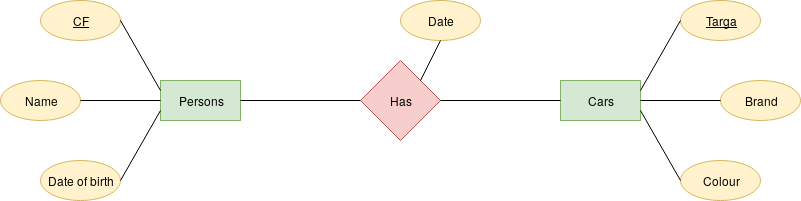
\includegraphics[width=\textwidth,keepaspectratio]{diagram1_00.png}
	\caption{The classic example}
	\label{diagram1_00}
\end{figure}

When we want to translate an Entity Relationship Diagram (ERD) into a Relation Model (RM) we have to follow certain rules, let's check them out.
\paragraph*{Rule \#1} Every entity is a table and its attributes are the table's columns.
\paragraph*{Rule \#2} Each relation is a table and its attributes are part of the table's columns; also the keys of the entities involved in the relation become columns and they are flagged as Foreign Keys (FK). The FKs must be the table Key.\\

Let's put this in practice:
\vskip 20pt
f
\begin{minipage}{0.45\textwidth}
	PERSONS
	\begin{table}[H]
		\centering
		\subimport{assets/tables/}{phc-pers.tex}
	\end{table}
	\texttt{PERSONS(\underline{CF}, Name, Birth date)}
\end{minipage}
\hspace{.1\textwidth}
\begin{minipage}{.45\textwidth}
	CARS
	\begin{table}[H]
		\centering
		\subimport{assets/tables/}{phc-cars}
	\end{table}
	\texttt{CARS(\underline{Targa}, Brand, Color)}
\end{minipage}
\vskip 20pt
That was pretty easy, wasn't it?\\
Now it's time to draw the relation table:
\vskip 20pt
\begin{minipage}{.7\textwidth}
	HAS
	\begin{table}[H]
		\subimport{assets/tables/}{phc-has}
	\end{table}
	\texttt{HAS(\underline{CF, Targa}, Date)}
\end{minipage}
\vskip 20pt
Well, that's clear. Now it's time to mix up things a little bit.
What if a car can't be owned by different people? (see \ref{diagram1_01})
\begin{figure}[H]
	\centering
	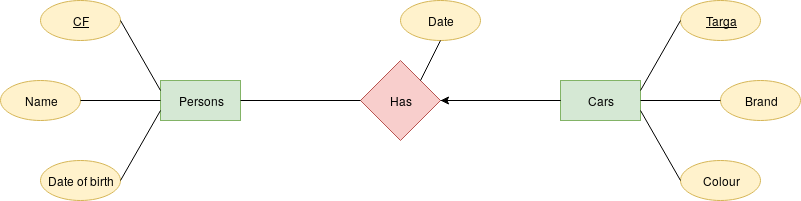
\includegraphics[width=\textwidth,keepaspectratio]{diagram1_01.png}
	\caption{A car now can have at most one owner}
	\label{diagram1_01}
\end{figure}
We must use only the Targa as key in HAS relation.
% TODO inserire qua una tabella con la rappresentazione di ciò??
\\
And what if we want the car to have also at least one owner? (see \ref{diagram1_02})
\begin{figure}[H]
	\centering
	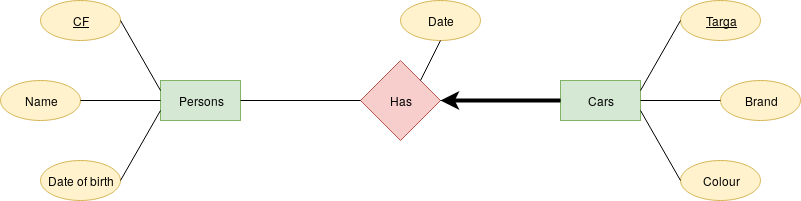
\includegraphics[width=\textwidth,keepaspectratio]{diagram1_02.png}
	\caption{A car now can have at most one owner}
	\label{diagram1_02}
\end{figure}
Now that a car must be owned by one (and only one) person it has no more sense to keep HAS table and CARS table divided: the smartest solution is to delete HAS table and introduce in CARS table two columns, one for Date and one for CF, which will be a FK. Last but not least the CF field must be mapped as \emph{not-null}.
That's the representation in RM:
\vskip 20pt
\begin{minipage}{.8\textwidth}
	CARS
	\begin{table}[H]
		\subimport{assets/tables/}{phc-cars_v2}
	\end{table}
	\texttt{CARS(\underline{Targa}, Brand, Color, CF, Date)}\\
	\texttt{	CF not null}\\
	\texttt{	CF Foreign Key to PERSONS}
\end{minipage}
\vskip 20pt

Going back to diagram \ref{diagram1_00}, what if I want to keep in memory all the times somenoe rent the same car?
Now I cannot do that because, being the Key,Targa cannot apear twice in the table.
The solution here is to use also Date as a Key.
But that's not fasiable because, as we stated in Rule \#2, only Keys of the entities are used as Key in the relation Table, and Date is not an entity; hence we have to redesign our diagram as
\begin{figure}[H]
	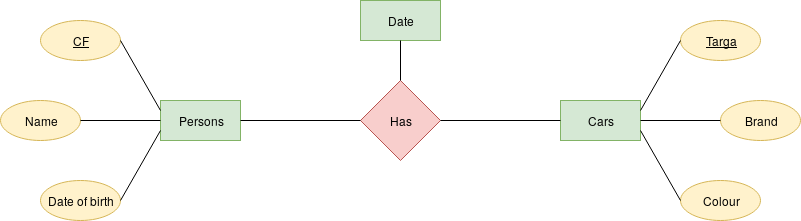
\includegraphics[width=\textwidth,keepaspectratio]{diagram1_03.png}
	\caption{Now Date is an entity}
	\label{diagram1_03}
\end{figure}
\vskip 20pt

Now we want that every Rent must have an Insurance, so we have to create a new entity called Insurance and link it to the Rent relation as this:
\begin{figure}[H]
	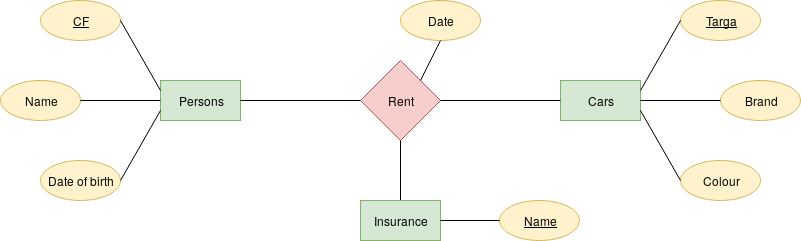
\includegraphics[width=\textwidth,keepaspectratio]{diagram1_04.png}
	\caption{We added Insurance as an entity}
	\texttt{RENT(\underline{Owner, Car, Name}, date)}\\
		\texttt{Owner FK to PERSONS}\\
		\texttt{Car FK to CARS}\\
		\texttt{Name FK to INSURANCE}
	\label{diagram1_04}
\end{figure}
\vskip 20pt

And now we decide that the Insurance is no more necessary for a Rent, how do we set it as a field hat can be null?
We have to link it to Rent with a relation, but we cant link two relations toghether: we must aggregate Persons, Rent and Car so that we can treat this set as an entity and then we can link to this new entity the Insurance with another relation (\ref{diagram1_05}).
\begin{figure}[H]
	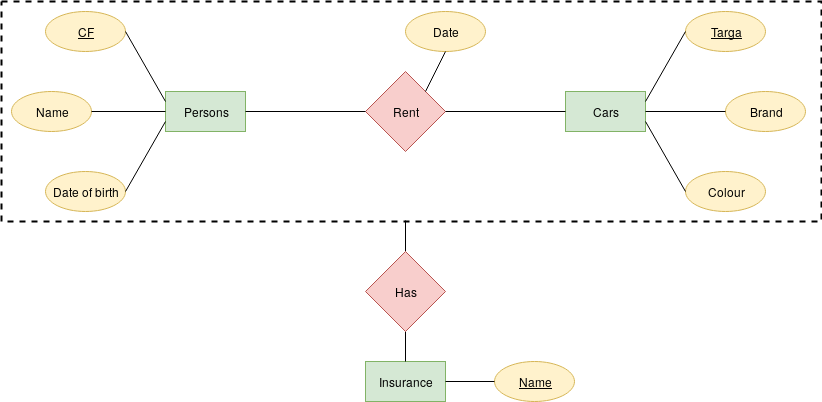
\includegraphics[width=\textwidth,keepaspectratio]{diagram1_05.png}
	\caption{We added Insurance as an entity}
	\label{diagram1_05}
\end{figure}
In this case what's going to be the key of Rent?
\vskip 10pt
\texttt{RENT(\underline{Owner, Car}, date)}\\
	\texttt{Owner FK to PERSONS}\\
	\texttt{Car FK to CARS}
\vskip 10pt
And which should be the Key of has?
Keeping in mind Rule \#2 we deduct that the keys of a relation must be the keys of the entities involved,marked as Foreign Key, therefore:
\vskip 10pt
\texttt{HAS(\underline{Owner, Car, Name})}\\
	\texttt{(Owner, Car) FK to RENT}\\
	\texttt{Name FK to INSURANCE}
\vskip 10pt
And now the last question for this example: what's the difference between \ref{diagram1_04} and \ref{diagram1_06}?
\begin{figure}[H]
	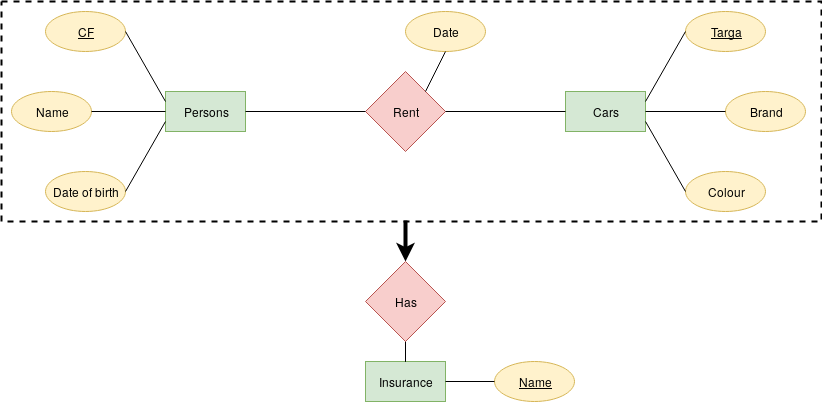
\includegraphics[width=\textwidth,keepaspectratio]{diagram1_06.png}
	\caption{Note the particular form of the diagram}
	\label{diagram1_06}
\end{figure}
The difference is:
\begin{itemize}
	\item In \ref{diagram1_04} you \emph{must} use Name as Key in RENT table, because Insurance is an entity involved in Rent relation (Rule \#2); therefore a person can rent the same car multiple times given that he uses a different insurance.\\
	\item In \ref{diagram1_06} you don't have to use Name as Key in RENT table, therefore it is not possible for a person to rent the same car with two different insurances (even if the insurance changes the key remains the same).
\end{itemize}

\section{Let's talk about inheritance}
It's time to see a little bit of inheritance, as always we're starting with an example:
\begin{figure}[H]
	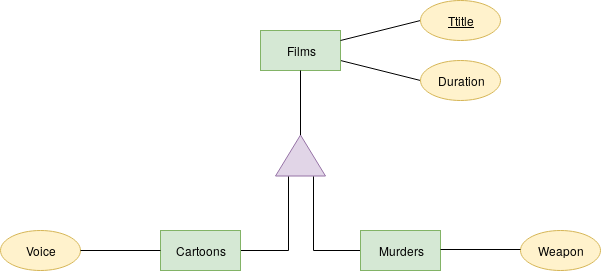
\includegraphics[width=\textwidth,keepaspectratio]{diagram2_00.png}
	\caption{An example of inheritance}
	\label{diagram2_00}
\end{figure}
There are three ways to translate ER inheritance into RM:
\begin{enumerate}
	\item The first approach is to have a different table for every entity, the tables of the children-entities will contain also the attributes inherited by the parent-entity.
	\vskip 5pt
	\texttt{FILMS(\underline{Title}, Duration)}\\
	\texttt{CARTOONS(\underline{Title}, Duration, Voice)   Title FK to FILMS}\\
	\texttt{MURDER(\underline{Title}, Duration, Weapon)   Title FK to FILMS}
	\vskip 5pt
	The bad aspect of this approach is that we store the different entity-types in different palces, for instance "Shrek" iss stored into CARTOONS table, therefore if we want to query the database by title and ask for "Shrek" we have to navigate trough all the three tables. Also if we want to query on how many films the database contains we will have to shearch in all the three tables.
	\item The second approach is to have a different table for every entity, but the tables of the children-entities contain only their specific attributes and the Key attribute of the parent-entity, which will be also the child-entity Key (Foreign Key).
	\vskip 5pt
	\texttt{FILMS(\underline{Title}, Duration)}\\
	\texttt{CARTOONS(\underline{Title}, Voice)   Title FK to FILMS}\\
	\texttt{MURDER(\underline{Title}, Weapon)   Title FK to FILMS}
	\vskip 5pt
	This approach is better because all the entities are stored in the FILMS table and therefore if we're querying, for instance, title or duration, we have to look only in the FILMS table. The films that are cartoons, like Shrek are going to be registered also in the CARTOONS table, and there we will find their voice attribute.
	The side effect of this approach is that when we query by, let's say, duration and voice we have to look into two different tables, and that's actually more complex than we need.
	\item The third approach is to store all the films iin the same table with all the attributes of the parent-entity and the children-entities, these will be filled with a \emph{null} value if the film stored won't be a cartoon or a murder.
	\vskip 5pt
	\texttt{FILMS(\underline{Title}, Duration, Voice, Weapon)}\\
	\texttt{Duration is not-null}\\
	\texttt{Voice and Weapon can be null}
	\vskip 5pt
	Thinking in a querying way that's the best approach, for every research in the database you have to navigate only trough a table.
\end{enumerate}

\chapter{Translating RM into ER}


\end{document}
